\documentclass{standalone}
\usepackage{tikz}

% for coil
\usetikzlibrary{decorations.pathmorphing}
%\usetikzlibrary{pattern}

\begin{document}
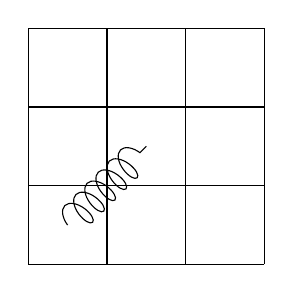
\begin{tikzpicture}
  \draw (0,0) grid (3,3);
  \draw[decoration={segment length=2mm, amplitude=2mm,coil},decorate] 
        (0.5,0.5) -- (1.5,1.5);
\end{tikzpicture}
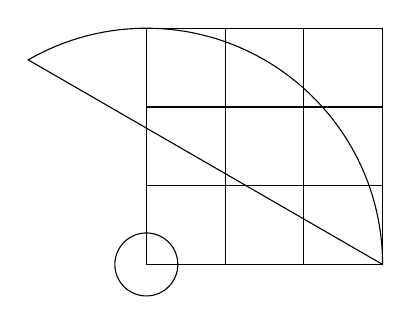
\begin{tikzpicture}
  \draw (0,0) grid (3,3);
  \draw (0,0) rectangle (2,3);
  \draw (0,0) circle [radius=0.4];
  \draw (3,0) arc (0:120:3) 
              -- cycle;
\end{tikzpicture}
\begin{tikzpicture}
  \draw[dashed] (2,2) circle (2);
  \fill[red](2+2*cos 30, 2+2*sin 30)circle(3pt);
  \fill[red](2+2*cos 120, 2+2*sin 120)circle(3pt);
\end{tikzpicture}

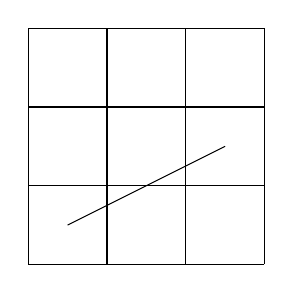
\begin{tikzpicture}
  \draw (0,0) grid (3,3);
  \coordinate (A) at (0.5,0.5);
  \coordinate (B) at (2.5,1.5);
  \draw (A) -- (B);
\end{tikzpicture}

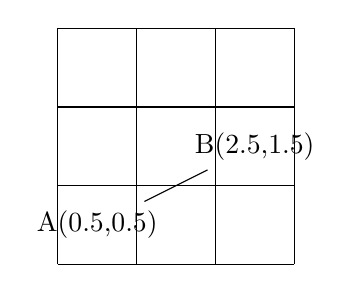
\begin{tikzpicture}
  \draw (0,0) grid (3,3);
  \node (A) at (0.5,0.5) {A(0.5,0.5)};
  \node (B) at (2.5,1.5) {B(2.5,1.5)};
  \draw (A) -- (B);
\end{tikzpicture}

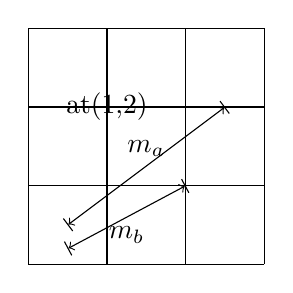
\begin{tikzpicture}
  \draw (0,0) grid (3,3);
  \node at (1,2) {at(1,2)};
  \draw[|<->|] (0.5,0.5) -- node[midway,above]{$m_a$} (2.5,2);
  \draw[|<->|] (0.5,0.2) -- (2,1) node[midway,below]{$ m_b$} ;
\end{tikzpicture}

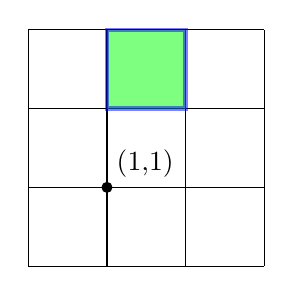
\begin{tikzpicture}
  \draw (0,0) grid (3,3);
  \fill (1,1) circle[radius=2pt] node[above right]{(1,1)};
  \filldraw[fill=green, opacity=0.5,draw=blue, ultra thick]
        (1,2) rectangle (2,3);

\end{tikzpicture}

\end{document}
